
%\documentclass[onecolumn,prl,nobalancelastpage,aps,10pt]{revtex4-1}

%\documentclass[rmp,preprint]{revtex4-1}

\documentclass[11pt]{article} % Try also "scrartcl" or "paper"
\linespread{1.5}
 \usepackage[margin=3cm]{geometry}   % to change margins
 \usepackage{titling,cite,subfig}             % Uncomment both to   
 \setlength{\droptitle}{0cm}     % change title position 
\title{%\vspace{-1.5cm}            % Another way to do
Feature Descriptors for Gait Analysis From Depth Sensors}
\usepackage{graphicx,bm,subfig,amsmath,amsfonts,listings,url}
\usepackage{gensymb}
\usepackage{color}
\usepackage{titlesec}
\usepackage{hyperref}
\usepackage[toc,page]{appendix}
 \usepackage{booktabs}
 \usepackage[table,xcdraw]{xcolor}
\titleclass{\subsubsubsection}{straight}[\subsection]
\usepackage{epstopdf}
\newcounter{subsubsubsection}[subsubsection]
\renewcommand\thesubsubsubsection{\thesubsubsection.\arabic{subsubsubsection}}
\renewcommand\theparagraph{\thesubsubsubsection.\arabic{paragraph}} % optional; useful if paragraphs are to be numbered

\titleformat{\subsubsubsection}
  {\normalfont\normalsize\bfseries}{\thesubsubsubsection}{1em}{}
\titlespacing*{\subsubsubsection}
{0pt}{3.25ex plus 1ex minus .2ex}{1.5ex plus .2ex}

\makeatletter
\renewcommand\paragraph{\@startsection{paragraph}{5}{\z@}%
  {3.25ex \@plus1ex \@minus.2ex}%
  {-1em}%
  {\normalfont\normalsize\bfseries}}
\renewcommand\subparagraph{\@startsection{subparagraph}{6}{\parindent}%
  {3.25ex \@plus1ex \@minus .2ex}%
  {-1em}%
  {\normalfont\normalsize\bfseries}}
\def\toclevel@subsubsubsection{4}
\def\toclevel@paragraph{5}
\def\toclevel@paragraph{6}
\def\l@subsubsubsection{\@dottedtocline{4}{7em}{4em}}
\def\l@paragraph{\@dottedtocline{5}{10em}{5em}}
\def\l@subparagraph{\@dottedtocline{6}{14em}{6em}}
\makeatother

\setcounter{secnumdepth}{4}
\setcounter{tocdepth}{4}


\usepackage{microtype}

%\renewcommand{\thesection}{\arabic{section}}
%\renewcommand{\thesubsection}{\thesection.\arabic{subsection}}
%\renewcommand{\thesubsubsection}{\thesubsection.\arabic{subsubsection}}
\DeclareMathOperator*{\argmin}{arg\,min}
% Fix references
\makeatletter
\renewcommand{\p@subsection}{}
\renewcommand{\p@subsubsection}{}
\makeatother

\usepackage{bibentry}

\newcommand{\comment}[1]{}
\begin{document}
\maketitle
\tableofcontents
\comment{

A statement of the aims and objectives of the project.


A description of the background and context of the project and its relation to work already done in the area. (Note that while you are free to re-use work from your research review here, it would normally be appropriate to tailor your earlier work to better suport the final contributions of the project. Typically you will include new related work which was found to be important, while excluding previously studied work which has become irrelevant, and modifying your earlier write-up with more or less detail, as required).



A description of the work carried out. This should include details of technical or scientific problems tackled, solutions proposed, and the design and development of software.



A description and analysis of results obtained.



A critical evaluation of the work. This is an analysis of the extent to which the project has achieved its objectives, and whether the choices that were made were, with hindsight, the best ones.
Suggestions on possible improvements and/or further work.


	Introduction:
		Discuss SPHERE, the need for in home gait analysis, references that show this is possible from kinect, 
	The existing pipeline:
		Kinect SDK skeletons... shotton et al.
		same as lit review, but go into more detail on the dimensionality reduction/manifold method
	

}

\title{Feature Descriptors for Gait Analysis from Depth Sensors}



\author{Ben Crabbe}

\date{\today}





\section{Introduction}

%SPHERE - a Sensor Platform for Healthcare in a Residential Environment, is a interdisciplinary research project being undertaken in Bristol which aims to help solve some of the problems currently faced by the healthcare system in the UK. The goal is to design a range of sensors to be fitted in residential environments that facilitate the care and rehabilitation of inhabitants. 
 %reference for some medical textbook?
%A Kinect Based Approach to Assist in the Diagnosis and Quantification of Parkinson’s Disease
%R. Torres, M. Huerta, R. Clotet, R. González, L. E. Sánchez, D. Rivas, M. Erazo
%Parkinson’s Disease (PD) is a degenerative process of the central nervous system. Its main body symptoms are tremors, rigidity, bradykinesia and walking difficulty. These symptoms may increase and so it is necessary to have a constant and successful evaluation, so the PD patient may receive the appropriate treatment. There are systems that enable the monitoring of tremors based on sensors, most of them attached to the patient’s body. Some such systems comprise accelerometers or use of Nintendo Wii Remote sensors (NWR). As a proposal that allows true portability, without the attachment of a single sensor to the patient’s body, or need for batteries, this paper introduces a pilot system that allows to diagnose PD and evaluate its severity using Kinect sensors.

%Problem- health home care gait analysis
Gait analysis plays an important part in the treatment and assessment of a number of medical conditions. At present gait analysis is usually performed through a combination of visual assessment by an experienced physiotherapist, automated methods such as marker based motion capture, pressure sensitive walkways or accelerometers. It requires patients to travel to a gait assessment laboratory which is far from ideal for patients who have difficulty walking. 

%Solution - Sphere gait analysis pipeline
This problem, and a range of other healthcare challenges, is being tackled through research and development by the SPHERE (a Sensor Platform for Healthcare in a Residential Environment) group in Bristol. An automatic, in home, gait analysis pipeline has been designed~\cite{Paiement,Tao} which assesses the quality of a subjects movement using inexpensive RGB-D cameras such as the Microsoft Kinect.

Currently this system uses joint position information captured by the OpenNI skeleton tracking software, based on the algorithm of~\cite{Shotton2011}. This skeleton tracking software infers the 3D coordinates of each of the body's relevant joints producing a $n_{joints} \times 3$ dimensional vector. This data is then processed using a manifold learning method, Diffusion maps~\cite{Coifman2006}, to reduce the dimensionality of the data. This method builds up a 3D representation of the types of body configurations displayed in a training dataset containing footage of the motion being measured. New skeleton data is then projected onto this manifold. This effectively parameterises the motion, removing the redundant information contained in the skeleton data, and enabling simple comparison of poses. \footnote{We will refer to the projected points in this space as the pose vector, and to the skeleton data as the body configuration or joint position vector.} Finally, a statistical model of normal gait is built up from the training data using these pose vectors. New data is compared with this model producing a quality score for both pose and dynamics on a frame-by-frame basis.

Since this system uses data driven, machine learning methods to learn both the manifold representation of pose and the model of normal motion, it can be applied to other types of movement quality assessment such a sports movement optimisation or physiotherapy exercise coaching. The system has been applied to a sitting-standing motion, to punching motions in boxing $^{how to site http://www.irc-sphere.ac.uk/work-package-2/movement-quality ?}$ and to people walking upstairs. 
%Limitation - doesn't work well in realisitic senarios

One issue currently limiting the effectiveness of this system is the fragility of the skeleton tracking software. This software was designed for controlling entertainment/gaming systems with the user viewed frontally, within a range of 1-4m and at a pitch angle near 0$\degree$. Outside of these conditions skeletons become noisy and unreliable. Typically only a small fraction of data recorded from a camera attached to the ceiling above the stairs is fit for use with the system. Increasing amount of usable data requires more intrusive camera placement which is to be avoided. The skeleton trackers also perform poorly when props are involved in the scene, for example grasping a banister or a ball often leads to erroneous joint positions for that arm. It also struggles to accurately record sitting/standing motions.
%Aims

The aim of this project is to develop a tailor made system for determining the reduced pose vector directly from RGB-D footage. To enable the flexibility of the rest of the system we require this new component to exhibit the same flexibility as the rest of the system by being able to record a wide range of motions. It should also work with an effective accuracy under the kinds of viewing angles produced by practical, unobtrusive, in home camera placements. This requires a data driven approach since the pose representation we wish to infer is not fixed, differing based on the body configurations presented in training data. %Simply we require a system that can be trained to regress from RGB-D image data to a point in a continuous 3d space.

The methodology we find most suited to this task is a convolutional neural network (CNN). CNN's are a supervised learning method for extracting features, e.g. the pose vector, from images. Given training images labelled with the expected output the network extracts progressively higher level features representations leading to the final pose vector. Following training the network is then able to generalise to unseen data, producing an output inferred from the examples it has seen. 

CNNs have been effectively applied to 2D~human~pose estimation from RGB images~\cite{Toshev,Pfister,Li2014,Jain2013a,Jain2014,Tompson,Tompson2014} where the positions of joints in the image plane were inferred. In~\cite{Accv2014} they were also applied to 3D joint position estimation from RGB, where they were shown to have reasonable accuracy from a range of viewing angles when trained with data captured by 4 cameras placed around the subjects. They have also been shown to benefit from depth depth data in the tasks of object detection~\cite{Gupta2014}, object pose estimation~\cite{Schwarz2015} and object recognition~\cite{Alexandre2013}. %However this will be the first work, to our knowledge, that attempts a form of human pose estimation using depth data. 

For assessing the effectiveness of our solution we focus on the staircase ascent motion, as this is the motion for which we possess the largest dataset. Refered to as the SPHERE staircase 2014 dataset~\cite{Paiement}, this includes 48 sequences of 12 individuals walking up stairs, captured by a Asus Xtion depth sensor placed at the top of the stairs in a frontal and downward-looking position. Each Frame provides RGB, depth and 3D joint position data. The accuracy of our predicted pose vectors are measured by computing the mean squared error (MSE) of the networks predicted pose vectors against the label values. We also measure the change in overall system performance (how well the measured gait quality score matches the score labelled by a trained physiotherapist). 



%State in general terms whether your project is more of Type I, II or III.
%Generally the project can be seen as type I since it 

%Explain the main novelty and added value.
To the best of our knowledge this project will be the first time that CNNs will be applied to a 3D human pose estimation task on RGB-D images. It will also be a novel combination of CNNs and manifold learning methods. We find that this makes the CNN easier to train and more effective overall since it has far less outputs to specify. If this is proved to be the case it could potentially be applied to other tasks that have been attempted with CNNs such as human action recognition.




\section{Background and Related Work}

\subsection{Depth Imaging}
\label{sec:Depth}


In depth images each pixel value represents the distance of that point from the camera. Depth images are unaffected by changes in lighting or human appearance. They provide a 3D map of the scene, making background-foreground separation far easier. These features can often simplify computer vision tasks, particularly human pose estimation~\cite{Chen2013}.

There are three main technologies used to produce depth images: Time~of~flight~(ToF) cameras, Stereo~imaging cameras and Structured~light cameras. It was not until the last~5~years that affordable good~quality RGB-D sensors came on the market and since then there has been an explosion in their use in the computer vision community~\cite{Han2013}.

The data in the SPHERE staircase dataset was captured using a Asus Xtion Pro Live which uses the structured light technology developed by Primesense (same as the Microsoft Kinect). It consists of an infrared laser emitter and an infrared camera, which together make up the depth sensor, and a RGB camera. An infrared laser is passed through a diffraction grating to produce a known pattern of dots that is projected onto the scene then reflected back and captured by the infrared camera. The measured pattern is compared to a reference pattern produced at a known distance of reflection, which has been stored during the calibration process. The surface of reflection being farther or nearer than the reference surface produces a shift in the pattern which is used to determine the depth value~\cite{Zhang2012a,Khoshelham2012a} as shown in figure \ref{fig:kinectMeasure}.

\begin{figure}
\centering
\includegraphics*[width=0.45\linewidth,clip]{kinectMeasure}%
\caption{The process by which depth is computed from triangulation of structured light. From \cite{Han2013}		\label{fig:kinectMeasure}}
\end{figure}

\subsubsection{Sensor Performance}
\label{sec:senPerf}

Most of the studies reported below have focused on the Microsoft Kinect however both sensors contain the same depth sensing system and have been shown to perform equivalently when compared~\cite{Gonzalez-Jorge2013}, hence we report the findings based off of the Kinect performance.

The range of the depth sensor is~0.8-3.5m with increasingly noisy or incomplete readings up to 8m. It has a~43$\degree$~vertical by~57$\degree$~horizontal field~of~view~\cite{Han2013}.

Stoyanov et al.~\cite{StoyanovTodorandLouloudiAthanasiaandAndreassonHenrikandLilienthal2011a} compare the performance of the Kinect with that of two other ToF depth imaging cameras (SwissRanger~SR-4000 and Fotonic~B70~ToF) assessing them against a ground truth of expensive and low fps laser depth scanner measurements. They find that within a range of 3.5m the Kinect outperforms the ToF sensors and is comparable to the laser scanner, outside of this range the accuracy falls considerably.

Both Khoshelham~\&~Elberink~\cite{Khoshelham2012a} and Smisek~et~al.~\cite{Smisek2011} have measured this effect experimentally comparing Kinect measurements with those from high performance laser scanners. They find that temporally fluctuating noise in the depth measurements increases quadratically with distance from the sensor so the depth precision decreases from around~±0.5cm~at~1m to~±7cm at~7m. Nguyen~et~al. shows that noise increases linearly with lateral distance, and is greatly increased on surfaces at greater than 70$\degree$~angles~\cite{Nguyen2012}. This last effect can lead to increased levels of noise around edges of humans. 

As well as noise the structured light sensors often return 'unknown' depth value pixels, known as holes, when the infrared receiver cannot read the reflected pattern properly. This can occur around the sides of foreground objects due to the slightly different viewing angles between the projector and camera as in regions 2~and~3 of figure~\ref{fig:kinectHoles4}, or when certain surface materials, such as human hair, interfere with the infrared pattern's reflection as in region~4 in figure~\ref{fig:kinectHoles3}. 
 \begin{figure}
\includegraphics*[width=1\linewidth,clip]{kinectHoles4}
\caption{Shows the holes in structured light depth data due to the different perspectives of IR projector and senor (regions~1~and~3) and due to the surface of reflection being roughly~5m away and at a large angle(region~2) From~\cite{Feng2013}		\label{fig:kinectHoles4}  } 
\end{figure}
 \begin{figure}
\includegraphics*[width=1\linewidth,clip]{kinectHoles3}
\caption{Shows the holes in depth data due abnormal reflections from certain glossy surfaces like the TV monitor and the subjects hair.  From~\cite{Feng2013}			\label{fig:kinectHoles3}  } 
\end{figure}

It should be noted that each of these studies mentioned above~\cite{Khoshelham2012a,Smisek2011,Nguyen2012} fail to consider the environmental factors in the quality of the measurement. Fiedler~\&~Muller \cite{Fiedler2013} show that air draft can cause changes of the depth values up to~21mm at a distance of~1.5m, and temperature variations cause changes up to~1.88mm~per~1$\degree$~C. They also find a temperature dependant drift in the position of objects captured by the RGB camera.

\subsection{Human Pose Estimation}

Human pose estimation (HPE) is generally considered as the task of measuring in 2D or 3D the joint positions of the human body. It is one of the most researched problems in computer vision because of its difficulty and due to its use in a variety of applications such as video surveillance, human–computer interaction, digital entertainment, sport science and medical applications.

This is a difficult task for a number of reasons. Firstly the human body has around 20 degrees of freedom~\cite{Forsyth2005}, producing a huge space of possible body configurations, many of which will cause some joints to be occluded when viewed from a single camera. Additional difficulties arise from the variety in human appearance and clothing, and from left right ambiguities. Traditional motion capture methods (MoCap) rely on markers attached to the subject and multiple cameras to overcome these issues. Whilst such systems can provide highly accurate pose data, their use is restricted to controlled environments using expensive and calibrated recording equipment which renders them unsuitable in many applications.

Monocular visual pose estimation methods (reviewed in \cite{Moeslund2006, Hen2009,Poppe2007,Sminchisescu2006,Liu2015}) are generally divided into two approaches (e.g. by \cite{Poppe2007}); model based (or generative) and model-free (or discriminative) approaches. Model based approaches use prior knowledge of human shape and kinematics such as fixed limb lengths and defined joint angle limits to cast the image to pose transformation as a nonlinear optimisation problem or probabilistically in terms of a likelihood function, i.e. given this image data (and sometimes previous frames pose knowledge) what is the most likely valid pose. Model-free approaches instead learn a direct mapping from image data to pose, generally requiring learning/example based methods to achieve this. Some 'hybrid' approaches combine the two using model-free methods as an initialiser to model based methods. 


\subsubsection{Human Pose Estimation Using Dimensionality Reduction}

With both of the above approaches there are significant issues posed by the high dimensionality of pose data. In model based approaches likelihood functions, which are usually multi-modal and non-Gaussian, require a randomised search~\cite{Sminchisescu2003}. Such searches in~20 dimensions are computationally expensive and often lead to super real time frame rates~\cite{Hen2009}. In model free approaches training data must account for the highly non-linear mapping between image and pose, which means that the pose space must be densely sampled in the training set. Densely sampling a 20 dimensional space, even just the parts that correspond to valid human motion, whilst also modelling all the invariant aspects such as body shapes, viewing angle etc requires an inordinate amount of data~\cite{Hen2009,Agarwal2006}.%Agarwal2006Recovering 3D human pose from monocular images

Although the full pose space is very large and high dimensional it has been shown e.g. in \cite{Brand1999,Elgammal2004} that when considering only movements in a well defined activity such as walking, then the pose data can be well represented by a low dimensional latent manifold. In a work closely related to our own Elgammal et al. \cite{Elgammal2004} use a Local Linear Embedding method to generate a 1D manifold representation (embedded within a 3D space)$^{(FIGURE?)}$ of a walking motion from single sequences of silhouette images. They use a Generalised Radial Basis Function interpolation framework~\cite{Poggio1990} (a form of neural network) to learn two mappings, one from the manifold to the silhouette image space and another from the manifold to full 3D joint positions. They then invert these mappings to extract points on the manifold from silhouettes and 3D joint positions from the points on the manifold. In contrast, our work builds the manifold representation from 3D joint position data, this has the benefit of the manifold representation not being tied to subject's visual appearance. This allows it to generalise naturally to multiple subjects, which is not the case in~\cite{Elgammal2004} (although they do introduce an solution for this problem in~\cite{Elgammal2004b}). It is also unlikely that this method could be used to capture abnormality in gait since defining an image to manifold transformation explicitly from the inverse constrains all input images to the poses contained in the original data. Elgammal et al. argue that learning a smooth mapping from examples is an ill-posed problem unless the mapping is constrained since the mapping will be undefined in other parts of the space. We address this issue in section~\ref{sec:abnormals}.

Brand \cite{Brand1999}, also inferred 3D pose from silhouettes using an intermediate manifold representation. He uses a maximum a posteriori estimation for mapping between the image and manifold space. This uses information across the whole input sequence to find the most likely and consistent solutions in order resolve the ambiguities in the many to many silhouette to pose mapping. A solution of this form is unacceptable in our case as one of the key features of the SPHERE system is online measurement.

Similarly Urtasan et al. \cite{Urtasun2005} used Scaled Gaussian Process Latent Variable Models (SGPLVM) \cite{Lawrence2004} on single training sequences (walking and a golf swing) labelled with 2D joint positions. These models build a low dimensional manifold, and simultaneously, a continuous mapping between this and the 2D joint positions. They use the low dimensional representation to facilitate efficient maximum a posteriori based tracking in this space. Again, this is only suitable as an offline solution. 

Tangkuampien and Suter \cite{Tangkuampien2006} used Kernel Principle Component Analysis (KPCA) to learn low dimensional representations of 3D joint positions, and separately using the same method, a low dimensional representation of silhouette images. They then learn a mapping between these spaces using Locally Linear Embedding (LLE) reconstruction. This has some similarity with using a CNN, where the image is transformed in to progressively more concise feature representations, before the regression takes place. The disadvantage of using LLE to perform the final transformation is that it is restricted to within the manifold space contained in pose training data. %As discussed above, our method has the benefit that it naturally maps unseen poses away from the manifold of the training data. This reduces the number of poses we must capture in our training data.

Rosales et al \cite{Rosales2000,Rosales2001} used 3D joint position data from a MoCap system to render synthetic training data from multiple angles. Hu moments were used to extract visual features from these (and real) images. Unsupervised learning was used to cluster 3D joint position data into areas of similar pose and a neural network was trained separately on each cluster to learn the mapping from visual features to pose. Using the developments in training of deep neural networks since this work we show that it is feasible to have a single CNN learn both the features best suited and the mapping to all poses. This removes the need for clustering and separate networks leading to a simpler, easily adaptable solution. Although their use of MoCap data as opposed to Kinect Skeletons for ground truth is a change we could expect to improve performance in our system. Similarly rendering synthetic training data from multiple angles would be a smart way of improving our viewing angle tolerance.

\subsubsection{Human Pose Estimation From Depth Images}

Challenging aspects of RGB HPE such as the variability in human appearance and scene lighting were greatly simplified with the advent of low cost commodity depth sensors. RGB-D also provides richer data for inferring 3D structure; human poses which could appear identical when projected onto the 2D image plane can be distinguished. Full body HPE methods from single depth images are reviewed in \cite{Helten2013}. With the Kinect/Xtion sensor and software packages (Kinect SDK or alternatively the open source OpenNI) low cost, flexible and reasonably accurate HPE is now available and has been employed in a huge variety of scientific applications~\cite{Han2013,Giovanni}.

The Kinect SDK and OpenNI skeleton trackers apply some inter-frame tracking algorithms to the single frame pose measurements of~\cite{Shotton2011}. In this work Shotton et al. leveraged a large mocap 3D joint position dataset which they re-targetted onto a variety of synthetic body models before rendering as if captured from a Kinect, simulating sensor noise, camera pose, and crop position. Producing synthetic depth images data is far simpler than in RGB since depth is far more invariant to subject clothing and appearance changes. Using these generated depth images and a ground truth labelling of each pixel as one of 31 body parts they trained a randomised regression forrest to perform this body part classification at each pixel using simple and computationally efficient pixel wise features. They then use these classifications to infer actual joint position through a simple averaging and mean shift procedure. The whole algorithm operates in real time on the computational resources allowed to them on the Xbox gaming consoles GPU. \cite{Shotton2013a} adapts this work by allowing pixel classifications of a number of surrounding joints to be used when estimating the joint position, rather than the single corresponding body part pixels as in~\cite{Shotton2011}. This is shown to improve the quality of the prediction for occluded joints. A similar use of mocap joint position data for rendering synthetic images from multiple views is suggested as an ideal way for increasing the view angle and subject invariance of our system.

Another discriminative method is \cite{Plagemann2010} where they find geodesic extrema (which are expected to correspond to the feet, hands and head) from Dijkstra’s algorithm on a graph produced by connecting all depth pixels in the image into a map. These points are identified (as hands feet or head) by applying local shape descriptors around the area. 

Other methods e.g.~\cite{Ye2011,Wei2011,Baak2011,Zhu2008} have focused on improving temporal smoothness of the measured pose by combining such discriminative methods with model based temporal tracking methods. 

In a recent attempt Chan et al \cite{Chan2014} use 3D point cloud information and propose a viewpoint and shape histogram feature based off these point clouds. This feature is then used to categorise the pose based on the action being performed using an introduced action mixed model. Each action is prescribed its own low dimensional manifold which allows a human pose database containing a limited amount of data to probabilistically infer the full pose.
%look at He2015




\subsection{Convolutional Neural Networks}

Convolutional Neural Networks (CNNs) are biologically inspired supervised learning systems for extracting features from images. Essentially their goal is to learn an approximation of the function
\begin{equation}
\boldsymbol{Y} = F(\boldsymbol{Z},\boldsymbol{W})
\label{eq:networkF}
\end{equation}
where~$\boldsymbol{Z}$ is an input image, the output~$\boldsymbol{Y}$ is the inferred pose vector for this image, and~$\boldsymbol{W}$ are the trainable parameters of the network. 
 
They consist of a set of filter maps, essentially matrices (or tensors if applying to multiple channels), which are applied repeatedly across the whole of the input. Each application of these filters produces an activation value which is the sum of each filter element multiplied by its corresponding input pixel value plus a shift term known as a bias. The filter is applied iteratively across the whole image, typically with some overlap. This builds up an `activation map' for that filter. With such a layer being comprised of a number of filters. The activations of each filter are stacked together, becoming the new image which is passed onto the next layer. This process is illustrated in figure \ref{fig:convnet}. This type of layer, known as Convolution layers, are typically followed by a non-linear function which is what enables the CNN to learn non-linear transformations such as the image to pose transformation we require. Although it is possible to stack convolutional layers on top of each other they are often followed by a pooling layer (also called subsampling). The idea of pooling is to reduce the spatial size from the previous layer as seen in figure~\ref{fig:pool}. Operating on each depth slice individually, i.e. each filters activation, the pooling window moves across the image taking the values of the elements in the input, conglomerating them using some operation, typically taking the max value as seen in the right hand side of figure~\ref{fig:pool}. CNNs also typically contain one or more fully connected layers at the end. Being fully connected means that rather than having a small filter applied repeatedly across the input, a number of filters of the same dimensions as the input are applied to the whole volume. This then outputs a~$1\times 1 \times K$ volume where~$K$ is the number of filters. This is then identical to regular neural networks where each unit in a layer is connected to every unit in the next. In our case, fully connected layers take the final high level feature representation from the rest of the network and perform the final regression to the pose vector. 

\begin{figure}
\includegraphics*[width=1\linewidth,clip]{convnet}
\caption{Shows a representation of the activations produced following a number of convolution layers, non-linearities (Rectified Linear Units, or ReLUs, are the function $max(0,x)$ and pooling layers. The network, an online demo from \cite{KarLects}, is classifying images from the CIFAR-10 dataset using the ConvnetJS library\protect\footnotemark. ) \label{fig:convnet}  }
\end{figure}
\footnotetext{http://cs.stanford.edu/people/karpathy/convnetjs/}

\begin{figure}
\includegraphics*[width=1\linewidth,clip]{pooling}
\caption{Shows the effect of pooling layers in a CNN.  From~\cite{KarLects} \label{fig:pool}  } 
\end{figure}

CNNs are trained using backpropagation and gradient descent. During training an error function is defined which quantifies the difference between the networks output and the desired output. In our case, as is typical of regression tasks, we use the euclidean distance between the two. Using the backpropagation algorithm~\cite{Rumelhart1986} the derivative of this error with respect to each parameter is found.  Then the values of each parameter are adjusted a small amount in the direction which reduces the error. In this way, over many training examples, the network converges on a minima in the error surface across the space of all parameter values.  A derivation of the backpropagation equations and further technical discussion of CNNs in general can be found in the preceding work on this project~\cite{Crabbe2015}.

An advantage of CNNs over traditional computer vision methods is that rather than prescribing a hand-engineered feature such as the depth disparity feature in~\cite{Shotton2011} or the view point and shape feature of~\cite{Chan2014}, the network is responsible for learning features itself based off the data. This presents a significant advantage in our application since features which might be good for measuring pose for one type of motion may not be useful for other motions. %

Deep CNNs have a proven capacity to learn a huge number of different visual representations. They have achieved great success in the International Large Scale Visual Recognition Challenge (ILSVRC, or ImageNet challenge) which is conducted each year and requires identification and localisation (separately) of 1000 different types of object. The work of~\cite{Krizhevsky2012} showed how deep networks could be trained by using ReLU non-linearities in place of the previous staple of tanh or logisitic functions, this over came the vanishing gradient problem that had previously made large network infeasible. Since then CNNs have achieved the best results in each task every year running, with every single participating team using them by 2014~\cite{Russakovsky}.

Training deep networks requires a large amount of data. Without this the network may begin to overfit the training data. When this occurs the errors for the network on inputs not in the training set, known as the test set, increases. It can be shown~\cite{Seung1992,Vapnik1994} that the difference between the errors on test set and those on the training set is related to both the size of the training set,~$P$, and the capacity,~$c$,  of the network i.e. 
\begin{equation}
E_{test}-E_{training} \propto \frac{c}{P}
\label{eq:errorCap}
\end{equation}
The capacity of the network is essentially the number of parameters being trained, which depends on the number of layers, the dimensions of the input images and the number of channels, the size and number of convolving filters and the way the filters and the pooling are applied. Increasing capacity will also decrease the size of~$\boldsymbol{E}_{training}$, hence there the aim in designing the network is to find the architecture which minimises both~$\boldsymbol{E}_{training}$ and~$\boldsymbol{E}_{test}-\boldsymbol{E}_{training}$ as far as possible~\cite{LeCun1998}.

Since ImageNet contains around 15 million training examples it has enabled the training of very large networks such as the 2014 winner GoogLeNet which had 22 layers~\cite{Szegedy2014}. In our case we are limited by the size of our dataset which contains a total of 6228 usable examples, many of which are practically identical due to being adjacent frames. A common method used to apply deep CNNs to tasks which lack large amounts of training data is to use a network pre-trained on a large dataset, typically ImageNet. Numerous studies~\cite{Sharif2014,Donahue2014,Oquab2014,Girshick2014,Yosinski2014} have shown ImageNet trained networks producing better results than randomly initialised networks in a variety of tasks, and also on depth data~\cite{Schwarz2015,Alexandre2013}. Typically the filters in the early layers are generic edge, corner or blob detectors which can be expected to generalise well to different tasks. In higher layers, as the spatial size of the input to each filter increases (due to pooling), more task specific representations are learnt. 

\subsubsection{Human Pose Estimation Using CNNs}

\label{sec:HpeCnn} 

Jain et al.~\cite{Jain2013a} were the first to apply CNNs to human pose estimation. They trained multiple small three layer networks to act as joint detectors with a separate network for each joint. Each network takes a small window of the full image as input. They are applied repeatedly with some overlap to produce probability map of the joint's estimated location. They then use a spatial model which enforces consistent and valid global pose estimates from the estimated joint locations. In~\cite{Jain2014} they extend their system to videos using RGB plus motion features e.g. optical flow. 

In a similar work Toshev and Szegedy~\cite{Toshev} used a multi resolution approach to find 2D joint locations. They used the architecture of~\cite{Krizhevsky2012} first applied to the full image at a low resolution. They then apply another network to a higher resolution image of just the area around the locations of the joints as determined by the first network. This successively refines the predictions. 

Li and Chan also measure 2D joint locations with a CNN. They use a single network with three convolution layers which they train for a pose regression and a joint detection simultaneously, sharing all convolution filters between tasks. They show that training for the extraneous task of joint detection consistently improves the accuracy of the regression task. In~\cite{Accv2014} they extend their work to 3D joint position measurements. They also compare the original multi task training with pre-training on joint detection before fine tuning on regression. They find little difference between the two but still show that the joint detection task consistently improves the regression performance. They show that the network produces reasonable position estimates even for completely occluded joints. 

Pfister et al.~\cite{Pfister} used the architecture of~\cite{Sermanet2013a} (a 2013 ILSVRC winner) to regress 2D upper body joint locations from RGB video. They experiment with using an ImageNet pre-trained model but find results are improved when training from scratch, a result echoed in this work. The found a their accuracy improved by 5\% after performing background subtraction on their data, a method we also adopt. They also experiment with using multiple frames as input, finding this gives only a modest 0.3\% improvement. 

Tompson et al.~\cite{Tompson2014}

Recently Belagiannis et al.~\cite{Belagiannis} showed that convergence times and final accuracy in HPE tasks can be improved by replacing the common L2/Euclidean loss function with a function that reduces the effect of outliers in the objective space. They state that the L2 loss functions give a disproportionally high weight to outliers which negatively effects the training procedure, reducing the generalisation ability and increasing the convergence times. They propose a new loss function, Tukey's biweight loss function, which acts to minimise the effect of outliers and show that employing this function improves results in better accuracy and convergence rates on 2D HPE task. This is an interesting finding which is especially relevant to this work where a noisy skeletons produce a significant number of outliers. Unfortunately this paper was not discovered until after most of the work was completed. A direction of future work will be to implement this loss function.



%To be finished...



\section{Methods}

\subsection{Data Preprocessing}
\label{sec:preprocessing}

The dataset used in this project (SPHERE-staircase2014~dataset~\cite{Paiement}) includes 48 sequences of 12 individuals walking up stairs, captured by a Asus Xtion depth sensor placed at the top of the stairs in a frontal and downward-looking position. It contains three types of abnormal gaits with lower-extremity musculoskeletal conditions, including freezing of gait and using a leading leg, left or right, in going up the stairs. All frames have been manually labelled as normal or abnormal by a qualified physiotherapist. There are 17 sequences of normal walking from 6 individuals and 31 sequences from the remaining 6 subjects with both normal and abnormal walking. The dataset contains a reasonable variation in body shape and appearance as can be seen in figure \ref{fig:subjects}.



\begin{figure}
\centering
\subfloat[Subject 1.		\label{fig:sub1} ]{{3
\includegraphics*[width=0.17\linewidth,clip]{depth_258.png} }}%
\qquad
\subfloat[Subject 2.	\label{fig:sub2} ]{{
\includegraphics*[width=0.17\linewidth,clip]{depth_186Adj.png} }}%
\qquad
\subfloat[Subject 3.   \label{fig:sub3} ]{{
\includegraphics*[width=0.17\linewidth,clip]{depth_122.png} }}%
\qquad
\subfloat[Subject 4. \label{fig:sub4} ]{{
\includegraphics*[width=0.17\linewidth,clip]{depth_286.png} }}%
\qquad
\subfloat[Subject 5. \label{fig:sub5} ]{{
\includegraphics*[width=0.17\linewidth,clip]{depth_260.png} }}%
\qquad
\subfloat[Subject 6. \label{fig:sub6} ]{{
\includegraphics*[width=0.17\linewidth,clip]{depth_229.png} }}%
\qquad
\subfloat[Subject 7. \label{fig:sub7} ]{{
\includegraphics*[width=0.17\linewidth,clip]{depth_171.png} }}%
\qquad
\subfloat[Subject 8. \label{fig:sub8} ]{{
\includegraphics*[width=0.17\linewidth,clip]{depth_175.png} }}%
\qquad
\subfloat[Subject 9. \label{fig:sub9} ]{{
\includegraphics*[width=0.17\linewidth,clip]{depth_280.png} }}%
\qquad
\subfloat[Subject 10. \label{fig:sub10} ]{{
\includegraphics*[width=0.17\linewidth,clip]{depth_265.png} }}%
\qquad
\subfloat[Subject 11. \label{fig:sub11} ]{{
\includegraphics*[width=0.17\linewidth,clip]{depth_252.png} }}%
\qquad
\subfloat[Subject 12. \label{fig:sub12} ]{{
\includegraphics*[width=0.17\linewidth,clip]{depth_221.png} }}%
\caption{The subjects contained in the SPHERE staircase 2014 dataset.}
\label{fig:subjects}
\end{figure}


% Please add the following required packages to your document preamble:
% \usepackage[table,xcdraw]{xcolor}
%% If you use beamer only pass "xcolor=table" option, i.e. \documentclass[xcolor=table]{beamer}
%\begin{table}[]
%\centering
%\begin{tabular}{lll}
%\hline
%Subject & Sequence                        & length                     \\ \hline
%1       & {\color[HTML]{333333} Normal 1} & {\color[HTML]{333333} 206} \\
%        & {\color[HTML]{333333} Normal 2} & {\color[HTML]{333333} 147} \\
%        & {\color[HTML]{333333} Normal 3} & {\color[HTML]{333333} 67}  \\ \hline
%2       & {\color[HTML]{333333} Normal 1} & {\color[HTML]{333333} 154} \\
%        & {\color[HTML]{333333} Normal 2} & {\color[HTML]{333333} 152} \\
%        & {\color[HTML]{333333} Normal 3} & {\color[HTML]{333333} 167} \\ \hline
%3       & Normal 1                        & 99                         \\
%        & Normal 2                        & 47                         \\ \hline
%4       & Normal 1                        & 174                        \\
%        & Normal 2                        & 74                         \\
%        & Normal 3                        & 173                        \\ \hline
%5       & Normal 1                        & 57                         \\
%        & Normal 2                        & 50                         \\
%        & Normal 3                        & 92                         \\ \hline
%6       & Normal 1                        & 65                         \\
%        & Normal 2                        & 102                        \\
%        & Normal 3                        & 106                        \\ \hline
%7       & Normal 1                        & 91                         \\
%        & Right Leg                       & 262                        \\
%        & Stop x 2                        & 151                        \\ \hline
%8       & Normal 1                        & 91                         \\
%        & Normal 2                        & 125                        \\
%        & Stop x 2                        & 205                        \\ \hline
%9       & Normal 1                        & 116                        \\
%        & Normal 2                        & 34                         \\
%        & Normal 3                        & 91                         \\
%        & Left Leg                        & 105                        \\
%        & Right Leg                       & 197                        \\
%        & Stop x 1                        & 158                        \\ \hline
%10      & Normal 1                        & 65                         \\
%        & Left Leg                        & 281                        \\
%        & Stop x 1                        & 172                        \\ \hline
%11      & Normal 1                        & 73                         \\
%        & Normal 2                        & 120                        \\
%        & Left Leg                        & 210                        \\
%        & Right Leg                       & 199                        \\
%        & Stop x 1                        & 172                        \\
%        & Stop x 2                        & 215                        \\ \hline
%12      & Normal 1                        & 114                        \\
%        & Normal 2                        & 92                         \\
%        & Normal 3                        & 101                        \\
%        & Left Leg                        & 233                        \\
%        & Right Leg                       & 259                        \\
%        & Stop X 1                        & 157                        \\
%        & Stop X 2                        & 207                        \\ \hline
%total:  &                                 & 6228                       \\
%        &                                 &                           
%\end{tabular}
%\caption{My caption}
%\label{my-label}
%\end{table}
Each example consists of the RGB image, the depth image and 3D joint position / skeleton data. Preprocessing is applied to each of these separately.

\subsubsection{Skeleton Preprocessing}

These processes were developed by the authors of~\cite{Paiement} and are a pre-requisite for the manifold learning stage of that work and this. First the Skeleton data is smoothed over time to reduce the large amount of noise. Each skeleton is scaled to the same height, rotated to face forwards and translated to the origin. Each skeleton is compared with a neutral reference pose;  a dissimilarity measure is computed  using the sum of squared distances between corresponding joints, standardised by a measure of the scale of the reference shape. Any frames where this dissimilarity is greater than 0.1 are discarded. These are generally frames from the beginning and end of sequences, where the subject is outside the sensors optimum range, and any particularly noisy periods in the middle. 

Specifically for this project we also take the mirror image of each skeleton. Combined with a mirror image of the depth image, this doubles our data. 

Now the collection of remaining skeletons is given to the manifold learning stage. The method used is Diffusion Maps~\cite{Coifman2006} with an adaptation to better handle the remaining noise and outliers present in the skeleton data. We refer to the original publications~\cite{Paiement} and~\cite{Tao} for a full technical description. In essence Diffusion Maps retains the relative distances between data in the reduced space of the data. \cite{Tao} analysed the quality assessment performance using 1,2,3,4, and 5 dimensional representations and concludes that a 3D representation is the most effective.

The set of data which is used in building the manifold determines its form. In the original works~\cite{Paiement} and~\cite{Tao} the authors used only the 'normal' sequences from the first 6 subjects. The manifold this produces is shown in figure \ref{fig:1-6manifoldNoFlips}. We initially worked with a manifold built from all sequences abnormal and normal from each of the 12 subjects. This produces a slightly different manifold shown in figure \ref{fig:1-12maniWFlips}. Once we switched to using the final manifold we observed an increase in accuracy of around 20\%. This shows that the form of the manifold can have a significant effect on the accuracy of the CNN, and therefore that these results for gait analysis may not be a reliable indication of performance on other movements and manifolds.

All results presented here after use the 2793 skeletons from the first 6 'normal' sequence subjects plus their horizontal flips to build the manifold, shown in figure \ref{fig:1-6manifoldWFlips}. The skeletons of the 31 sequences from the other 6 subjects (and their flips) are then projected onto the manifold (again, see \cite{Paiement} and~\cite{Tao} for details). Interestingly the flipped skeletons produce a manifold coordinate precisely equal to the non flipped version but with the first component negated. This suggests that each of the three components of the manifold are tied with the 3 regular spacial dimensions of the skeletons, although there is no guarantee of this with the Diffusion Maps method. 

To illustrate the meaning of the manifold coordinates the skeletons placed at the 3 corners are shown in figure \ref{fig:skelToManifod}. Generally the normal gait sequences follow paths across the dense quarter sphere shaped surface with the frame of maximal left and right knee flex occurring at the maximum and minimum of first coordinate. The second dimension, plotted horizontally in figure \ref{fig:skelToManifod}, seems to measure the vertical distance between skeletons. The skeleton with raised knees occur near its minimal value and at its maximum we find elongated skeletons which are measured erroneously when subjects are very close to the camera but just survive the cut on skeleton disimilarity. During processing of the images we remove these images from the dataset which results in the removal of most of the points which lie at this end of the manifold, as shown in figure \ref{manifoldAfterImageProcessing}. 

The meaning of the 3rd manifold coordinate is less clear. Figure \ref{fig:skelsZcomp} compares skeletons of minimum and maximum values for points of equal Y[0], Y[1], we are able to find no discernible pattern. This is reflected by the CNN as we find it far less accurate in this coordinate than the others. However this coordinate is somewhat subject specific, as seen in figure \ref{fig:subjectsOnManifold}, with each subject found to traverse the quater-sphere surface with a Y[2] range smaller than that of the full manifold. We find that fine tuning our networks on additional sequences of the subject being tested improves results by 28\%. 
%exlain how here or leave till later?



%will do a figure with skeletons -> manifold labelled and discuss what the 3 dimension represent.

\begin{figure}
\centering
\subfloat[The manifold produced by normal sequences of subjects 1-6. This was the form used in~\cite{Paiement}. We connect points from neighbouring frames for better visualisation of the structure.	\label{fig:1-6manifoldNoFlips} ]{{
\includegraphics*[trim={2cm 8cm 2cm 10cm},clip,width=0.45\linewidth,clip]{1-6maniNoFlips.pdf} }}%
\qquad
\subfloat[The manifold produced by normal sequences of subjects 1-6 including their horizontal flips. This was the form used in this work.\label{fig:1-6manifoldWFlips}]{{
\includegraphics*[trim={2cm 8cm 3cm 10cm},clip,width=0.45\linewidth,clip]{1-6maniWFlips} }}%
\qquad
\subfloat[The manifold produced by all sequences including their flips. The larger variation in the z component (the vertical axis in the figure) led to lower network accuracy and incorrect normality analysis.  \label{fig:1-12maniWFlips} ]{{
\includegraphics*[trim={0cm 5cm 0cm 9cm},clip,width=0.7\linewidth,clip]{1-12maniWFlips.pdf}}}%
\caption{}
\label{fig:manifolds}
\end{figure}


\begin{figure}
\centering
\includegraphics*[trim={1cm 18cm 1cm 1cm},clip,width=0.96\linewidth,clip]{skelToManifod} 
\caption{Normal gait sequences trace paths between the two corners on the right, with the postion of maximal knee flex the turning point. The left most coner of the manifold consists of elongated skeletons which tend to be measured when the subject is too close to the sensor. }
\label{fig:skelToManifod}
\end{figure}

\begin{figure}
\centering
\includegraphics*[trim={0 5cm 0 9cm},clip,width=0.75\linewidth,clip]{manifoldAfterImageProcessing.pdf} 
\caption{After image pre-processing we retain only those points shown in blue. }
\label{fig:manifoldAfterImageProcessing}
\end{figure}

\begin{figure}
\centering
\subfloat[Red skeleton has Y[2] = -0.2211, black has Y[2] = 0.1888\label{fig:-1.165-0.6517} ]{{
\includegraphics*[trim={3cm 8cm 3cm 8cm},clip,width=0.45\linewidth,clip]{-1_165-0_6517} }}%
\qquad
\subfloat[Red skeleton has Y[2] = -0.0499 , black has Y[2] = 0.4803.\label{fig:0.9485,-0.1622}]{{
\includegraphics*[trim={3cm 8cm 3cm 8cm},clip,width=0.45\linewidth,clip]{0_9485,-0_1622} }}%
\caption{Shows skeletons within 0.02 of the same Y[0],Y[1] postition but with maximum difference in Y[3]. We find no clear difference between the Skeleton of minimum and maximum Y[2]. This is reflected by the CNN which measures this coordinate with a lower accuracy than the first two.}
\label{fig:skelsZcomp}
\end{figure}

\begin{figure}
\centering
\includegraphics*[trim={0 5cm 0 7cm},clip,width=0.75\linewidth,clip]{subjectsOnManifold.pdf} 
\caption{Each normal sequence of the first 6 subjects plotted in a different colour. We observe that Y[2] coordinates for each subject tend to ramain within a sub-region of full range. This finding promoted the use of subject finetuning which improves the accuracy of Y[2] predictions. }
\label{fig:subjectsOnManifold}
\end{figure}













\subsubsection{Depth Preprocessing}

%will add all scripts mentioned into appendix
%will add a preprocesing pipeline figure
As described in section \ref{sec:senPerf} depth images are generally incomplete and noisy. We first fill holes in the data using a simple method which iteratively paints in the maximum pixel values from the neighbouring cells. We initially experimented with using the method of \cite{Camplani2012a} which combines noise filtering and hole filling. However the version that we accessed did not use the motion detection and segmentation components. In practise we found that the quality of the filled and filtered depth maps produced by this version were inferior to those produced by the simple method.  \cite{Camplani2012a}'s method also required far longer processing times ~1 week for the full set as opposed to a 20 minutes for the simple method. 


\begin{figure}
\centering
\subfloat[Typical image before hole filling.		\label{fig:depthWithHoles} ]{{
\includegraphics*[width=0.4\linewidth,clip]{depth_334.png} }}%
\qquad
\subfloat[Filter and filled using a simplifed version of~\cite{Camplani2012a}. \label{fig:camplaniCleaned} ]{{
\includegraphics*[width=0.4\linewidth,clip]{clean_depth_334.png} }}%
\qquad
\subfloat[Filled using max fill method.   \label{fig:quickFilled} ]{{
\includegraphics*[width=0.4\linewidth,clip]{qFilled_334.png} }}%
\caption{A comparison of hole filling methods. We use the max fill method. }
\label{fig:filtering}
\end{figure}



We then perform background subtraction on the filled depth images. We employed the C++ BGS library~\cite{bgslibrary} and tested each of the provided methods on our data. For all methods some initial set of background frames at the beginning of the sequence were required to achieve satisfactory results. The best results were achieved using the dp/DPZivkovicAGMMBGS method which implements~\cite{Zivkovic2004}. 


We found that the foreground masks produced often mistook sensor noise for moving objects. To fix this problem we apply a simple cleaning procedure to the masks which takes only the largest collection of positive pixels. This discards the small noise related blobs. We also apply a small erosion and dilation to get rid of noise effects connected to the largest blob. There is also problems correctly identifying the feet of the subjects since the floor is at approximately equal depth and therefore the same colour in the depth image. The masks generally only extend to around the mid point of the shin. For some subjects feet can appear mid stride when raised high enough from the ground to be distinguishable. We also attempted using the RGB images to improve extraction of the feet. However most subjects are wearing dark coloured shoes which did not differentiate well from the colour of the stairs, meaning the results we just as poor as for the depth, with additional issues in other parts of the images where clothing matched the colour of the walls. Additionally the subtraction fails badly on some frames, particularly towards the end of a sequence. These images are discarded. 

We then take the cleaned mask and extract the foreground containing the human figure from the depth image. In some cases patches of background get included around the edges of the mask. We remove any pixels which have values greater than two standard deviations from the mean of the foreground. Due to the perspective of the camera the depth values of the of the foreground increase towards the feet of the subject, therefore if this cut is too strict we begin to loose valid pixels near the feet. To avoid this whilst still removing all background pixels from the rest of the image we select only the top 75\% of the figure and apply a more stringent cut. 

Since all skeleton data was scaled and transformed to a common point we do the same to the depth data. We normalise the mean depth values of the of each image by finding the mean depth value of a small region near the subjects waist. Using only this region gives an accurate indication of the distance of the subject from the camera rather than transient effects such as arm swing. This value is subtracted from all foreground pixels before all being scaled to 0.5. 

Next we crop the background area from each image so that each is left with the average width to height ratio of the full dataset which is 0.504.

We then try to normalise the position of the figure within the image. There are two issues with the data which make this a necessary step, firstly the length of lower leg included in the masks varies from frame to frame, secondly there are a number of sequences in which the head of the subject leaves the camera's field of view during the middle of the ascent. Without fixing this problem the scale of the subjects in the images changes depending on how much of them was captured in the mask, which would mean the network would be required to learn an invariance to scale. In general we developed these preprocessing procedures to reduce the amount of invariance the network is required to learn. To fix this we try and identify the position of the shoulders; the width of the mask as a function of height in the image was found across the full dataset, the point greatest curvature was determined to lie at a width of 0.65 of the full image width (after initial cropping). We therefore define the point at which the the width of the mask exceeds this value as the shoulders. From this we find the position of the shoulders in each image. We found the mean position of the shoulders in all non-headless images to be 0.22 of the full image height. Then each image is rescaled, adding additional pixels of background so that the position of the shoulders occurs at exactly 0.22. If the initial shoulder position was less than 0.22 then we assume the image is missing part of its head and rows are added to the top, if it is greater than 0.22 we assume it misses more leg than usual and rows are added to the bottom. Whilst this doesn't recreate the actual foreground pixels of the legs or head, it does mean that the foreground pixels for each intact body part do occupy roughly the same position in the images. One limitation of this method is that it is difficult to handle images which lack both head and legs. We attempt to deal with this by storing the mean number of rows added to the bottom of the image across the sequence. Then if we find on the next frame that we are missing rows from the top (i.e. part of the head is missing) then we continue to add the mean number of rows to the bottom.

Next we adjust the colour balance of the image. Initially we used the basic scaled depth values and a black background. Analysis of the activations produced by the first layer filters of an ImageNet pre-trained network on this type of input , shown in figure \ref{fig:blackBGactiv}, seemed to indicate that depth information was not being extracted effectively. ImageNet first layer filters, shown in figure \ref{fig:layer1filts}, generally respond to edges. It is clear that the very small differences in depth between parts of the body will produce far smaller activations than the huge difference between the figure and the black background. To encourage the network to focus on the smaller edges we tried setting the background of the images to the mean depth value around the waist of the subject, as shown in figure \ref{fig:meanBG}. However after training until convergence the network seemed to have discarded most of the filters activations rather than adjusting to them as is seen in \ref{fig:meanBGactiv}. Finally we used histogram equalisation to increase the differences in depth values within the figure. We use a background value of 0.82 of the mean value at the subjects waist as this was slightly less than minimum value any valid foreground pixels seen in the dataset. This results in the largest spread possible in the foreground depth values without ever having a foreground value at a colour darker than the background. This scheme seems to achieve the desired result of allowing interior depth values and edges to be preserved through the first convolution layer as seen in figure \ref{adjustedNorm1}.

Finally, we remove images from the beginning and end of sequences where the subject is rotating or is very close to the camera as these are generally inaccurate and also because their are so few of these frames that they represent rare outliers in the dataset. The presence of such rare examples in the training data has been shown to hinder final network performance by \cite{Belagiannis}. 


\begin{figure}
\centering
\subfloat[Initial colouring scheme.		\label{fig:blackBG} ]{{
\includegraphics*[width=0.17\linewidth,clip]{depth_186.png} }}%
\qquad
\subfloat[Mean background method.	\label{fig:meanBG} ]{{
\includegraphics*[width=0.17\linewidth,clip]{depth_186Mbg.png} }}%
\qquad
\subfloat[Final scheme.   \label{fig:adjusted} ]{{
\includegraphics*[width=0.17\linewidth,clip]{depth_186Adj.png} }}%
\qquad
\subfloat[Pre-processed RGB \label{fig:rgb} ]{{
\includegraphics*[width=0.17\linewidth,clip]{img_186.png} }}%
\caption{}
\label{fig:colourschemes}
\end{figure}

\begin{figure}
\centering
\subfloat[The filters in conv1 of a imagenet pre-trained then finetuned AlexNet \cite{Krizhevsky2012}.	\label{fig:layer1filts} ]{{
\includegraphics*[width=0.45\linewidth,clip]{filters} }}%
\qquad
\subfloat[Initial colouring scheme		\label{fig:blackBGactiv} ]{{
\includegraphics*[width=0.45\linewidth,clip]{blackBGnorm1blob} }}%
\qquad
\subfloat[Mean background method	\label{fig:meanBGactiv} ]{{
\includegraphics*[width=0.45\linewidth,clip]{meanBGnorm1} }}%
\qquad
\subfloat[Final scheme   \label{fig:adjustedActiv} ]{{
\includegraphics*[width=0.45\linewidth,clip]{adjustedNorm1} }}%
\caption{The activations produced by the first layer filters for each of the colour schemes of figure \ref{fig:colourschemes}.  }
\label{fig:colourschemeActivations}
\end{figure}

A common pre-processing step when working with CNNs is to subtract the mean image of the training data (i.e. the mean value of each pixel) from each image. This is supposed to speed up training for reasons detailed in~\cite{LeCun1998a,Bottou2010,LeCun2012}. After testing the accuracy of the network's trained on such mean subtracted data we found that this operation actually decreased the performance as shown in figure \ref{fig:meanSubComp}. However this test was only conducted on an ImageNet pre-trained AlexNet (see section\ref{sec:alexNet}) , we have not studied the effect when training from scratch.

\begin{figure}
\includegraphics*[width=0.9\linewidth,clip]{meanSubComp.png} %
\caption{The accuracy of network predictions was seen to decrease when using mean subtracted data, hence we abandon this common practise.}
\label{fig:meanSubComp}
\end{figure}

\begin{figure}
	% GNUPLOT: LaTeX picture with Postscript
\begingroup
  \makeatletter
  \providecommand\color[2][]{%
    \GenericError{(gnuplot) \space\space\space\@spaces}{%
      Package color not loaded in conjunction with
      terminal option `colourtext'%
    }{See the gnuplot documentation for explanation.%
    }{Either use 'blacktext' in gnuplot or load the package
      color.sty in LaTeX.}%
    \renewcommand\color[2][]{}%
  }%
  \providecommand\includegraphics[2][]{%
    \GenericError{(gnuplot) \space\space\space\@spaces}{%
      Package graphicx or graphics not loaded%
    }{See the gnuplot documentation for explanation.%
    }{The gnuplot epslatex terminal needs graphicx.sty or graphics.sty.}%
    \renewcommand\includegraphics[2][]{}%
  }%
  \providecommand\rotatebox[2]{#2}%
  \@ifundefined{ifGPcolor}{%
    \newif\ifGPcolor
    \GPcolortrue
  }{}%
  \@ifundefined{ifGPblacktext}{%
    \newif\ifGPblacktext
    \GPblacktextfalse
  }{}%
  % define a \g@addto@macro without @ in the name:
  \let\gplgaddtomacro\g@addto@macro
  % define empty templates for all commands taking text:
  \gdef\gplbacktext{}%
  \gdef\gplfronttext{}%
  \makeatother
  \ifGPblacktext
    % no textcolor at all
    \def\colorrgb#1{}%
    \def\colorgray#1{}%
  \else
    % gray or color?
    \ifGPcolor
      \def\colorrgb#1{\color[rgb]{#1}}%
      \def\colorgray#1{\color[gray]{#1}}%
      \expandafter\def\csname LTw\endcsname{\color{white}}%
      \expandafter\def\csname LTb\endcsname{\color{black}}%
      \expandafter\def\csname LTa\endcsname{\color{black}}%
      \expandafter\def\csname LT0\endcsname{\color[rgb]{1,0,0}}%
      \expandafter\def\csname LT1\endcsname{\color[rgb]{0,1,0}}%
      \expandafter\def\csname LT2\endcsname{\color[rgb]{0,0,1}}%
      \expandafter\def\csname LT3\endcsname{\color[rgb]{1,0,1}}%
      \expandafter\def\csname LT4\endcsname{\color[rgb]{0,1,1}}%
      \expandafter\def\csname LT5\endcsname{\color[rgb]{1,1,0}}%
      \expandafter\def\csname LT6\endcsname{\color[rgb]{0,0,0}}%
      \expandafter\def\csname LT7\endcsname{\color[rgb]{1,0.3,0}}%
      \expandafter\def\csname LT8\endcsname{\color[rgb]{0.5,0.5,0.5}}%
    \else
      % gray
      \def\colorrgb#1{\color{black}}%
      \def\colorgray#1{\color[gray]{#1}}%
      \expandafter\def\csname LTw\endcsname{\color{white}}%
      \expandafter\def\csname LTb\endcsname{\color{black}}%
      \expandafter\def\csname LTa\endcsname{\color{black}}%
      \expandafter\def\csname LT0\endcsname{\color{black}}%
      \expandafter\def\csname LT1\endcsname{\color{black}}%
      \expandafter\def\csname LT2\endcsname{\color{black}}%
      \expandafter\def\csname LT3\endcsname{\color{black}}%
      \expandafter\def\csname LT4\endcsname{\color{black}}%
      \expandafter\def\csname LT5\endcsname{\color{black}}%
      \expandafter\def\csname LT6\endcsname{\color{black}}%
      \expandafter\def\csname LT7\endcsname{\color{black}}%
      \expandafter\def\csname LT8\endcsname{\color{black}}%
    \fi
  \fi
  \setlength{\unitlength}{0.0500bp}%
  \begin{picture}(8640.00,4320.00)%
    \gplgaddtomacro\gplbacktext{%
      \csname LTb\endcsname%
      \put(946,704){\makebox(0,0)[r]{\strut{} 0}}%
      \put(946,1374){\makebox(0,0)[r]{\strut{} 0.2}}%
      \put(946,2044){\makebox(0,0)[r]{\strut{} 0.4}}%
      \put(946,2715){\makebox(0,0)[r]{\strut{} 0.6}}%
      \put(946,3385){\makebox(0,0)[r]{\strut{} 0.8}}%
      \put(946,4055){\makebox(0,0)[r]{\strut{} 1}}%
      \put(1078,484){\makebox(0,0){\strut{} 0}}%
      \put(2102,484){\makebox(0,0){\strut{} 5000}}%
      \put(3125,484){\makebox(0,0){\strut{} 10000}}%
      \put(4149,484){\makebox(0,0){\strut{} 15000}}%
      \put(5172,484){\makebox(0,0){\strut{} 20000}}%
      \put(6196,484){\makebox(0,0){\strut{} 25000}}%
      \put(7219,484){\makebox(0,0){\strut{} 30000}}%
      \put(8243,484){\makebox(0,0){\strut{} 35000}}%
      \put(176,2379){\rotatebox{-270}{\makebox(0,0){\strut{}Validation Loss (l2 norm)}}}%
      \put(4660,154){\makebox(0,0){\strut{}Iterations}}%
      \put(4660,3945){\makebox(0,0){\strut{}}}%
    }%
    \gplgaddtomacro\gplfronttext{%
      \csname LTb\endcsname%
      \put(7256,3882){\makebox(0,0)[r]{\strut{}mean sub}}%
      \csname LTb\endcsname%
      \put(7256,3662){\makebox(0,0)[r]{\strut{}no mean sub}}%
    }%
    \gplbacktext
    \put(0,0){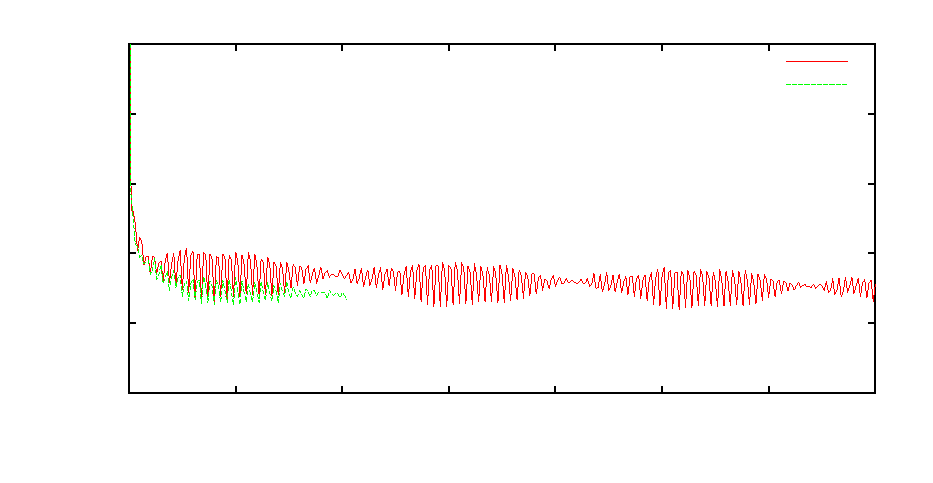
\includegraphics{introduction}}%
    \gplfronttext
  \end{picture}%
\endgroup
 
\end{figure}

\subsubsection{RGB Pre-processing}

For RGB images we applied the foreground masks retrieved from the corresponding depth images and then applied clipping and scaling in the same manner as the depth images. The result is shown in \ref{fig:rgb}. 

We measured the accuracy of an ImageNet pre-trained AlexNet (see section\ref{sec:alexNet}), which requires a 3 channelled input image, when using the RGB images only, the depth image replicated for each of the 3 channels only, and a combination of the two which consisted of 1 channel of the average of red and green, 1 channel of green and blue averaged and the depth in the final channel. As is shown in figure \ref{fig:rgbdcomp} the replicated depth was shown to produce the most accurate regression. All other results reported here use a pure depth input image. 

\begin{figure}
\includegraphics*[width=0.9\linewidth,clip]{rgb-dComp.png} %
\caption{Network accuracy when using the RGB images only, the depth image replicated for each of the 3 channels only, and a combination of the two which consisted of 1 chanel of the average of red and green, 1 channel of green and blue averaged and the depth in the final channel. }
\label{fig:rgbdcomp}
\end{figure}





\subsection{Software}

We use the open source CNN library Caffe~\cite{Jia2014} which is common among researchers including~\cite{Chen, Pfister,Girshick2014,Springenberg2015,Schwarz2015,Simonyan2015,Wang2015}. 

Caffe requires datasets to be in certain formats for training. When using multi-dimensional labels, as in our case, you are constrained to using a HDF5 formatted~\cite{Folk2011} dataset. 

One disadvantage of this is that automated shuffling options are not available as in the other dataset formats. Shuffling training examples is important for achieving the best training results in the shortest times. When training each adjustment to the network's parameters is proportional to the error on the last example. If the network is shown each ascent sequence in order the errors between each consecutive frame will be small since they contain very similar images and poses. Therefore we will waste lots of iterations making small updates. Since the HDF5 input layer in Caffe doesn't provide an automated shuffling we have to pre-shuffle the images and labels before storing them.

\subsection{Architecture}



\label{sec:alexNet}

%add figure
The architecture used, shown in figure \ref{fig:alexNet}, is a version of that which won the 2012 ILSVRC~\cite{Krizhevsky2012}. It consists of 5 convolutional layers, the 1st, 2nd and 5th of which are followed by max pooling layers. 

\begin{figure}
\centering
\includegraphics*[width=\linewidth,trim={0cm 0cm 0.78cm 12cm},clip]{alexNet} 
\caption{ The achitecture of~\cite{Krizhevsky2012} is used.\label{fig:alexNet}}
\end{figure}



This network also features Local Response Normalisation (LRN) layers. These normalise the values of each filter's activation with respect to the others in the same spatial position. Each activation is divided by
\begin{equation}
(1 + \frac{\alpha}{n} \sum_i^n x_i^2)^\beta
\end{equation}
where $x_i$ are the activations of filter $i$ at the same position. $n$, $\alpha$ and $\beta$ are adjustable parameters, which we leave unchanged from those used by ~\cite{Krizhevsky2012} at 5, 0.0001 and 0.75 respectively. The effect of this operation on our data is shown in figure \ref{fig:LRN}. 

\begin{figure}
\centering
\subfloat[The activations before LRN.	\label{fig:conv1} ]{{
\includegraphics*[width=0.45\linewidth,clip]{conv1} }}%
\qquad
\subfloat[And after	\label{fig:norm1} ]{{
\includegraphics*[width=0.45\linewidth,clip]{norm1} }}%
\caption{ }
\label{fig:LRN}
\end{figure}

To adapt this network for regression we replace the final fully connected layer with a 3 element layer which produces our final predicted pose vector. The Softmax loss function is replaced with an Euclidean loss which computes the l2-norm between this final vector and the label.

One advantage of using this architecture is that we can begin training from the weights trained on ImageNet before fine tuning on our smaller dataset. We tested the networks performance under 3 of these initialisation schemes with all other parameters fixed: 1) using the pre-trained weights for all layers, 2) using the pre-trained weights only on the first two convolution layers with a random initialisation on the others and 3) using a full random initialisation. We found that using imageNet weights in all layers significantly hindered the final performance as shown in \ref{fig:alexNetpre}. Schemes 2 and 3 produced very similar results, with scheme 2 having slightly better performance at some points earlier in the training. We use scheme 2 for our final results.


\begin{figure}
\centering
\includegraphics*[width=0.9\linewidth,clip]{AlexNetInitComploss.png} 
\caption{Shows a validation set loss for various pre-training schemes. We find that begining training from ImageNet pretrained weights throughout the network hinders performance. Using pre-trained weights only in the first two layers produced the best results. We use this strategy for our final tests. \label{fig:alexNetpre}}
\end{figure}

We also experimented with other architectures including VGG-S~\cite{Simonyan2015} the 2014 ILSVRC 2nd place model which has been shown to generalise better to other tasks than any other architecture~\cite{Chatfield2014}. However this deep 19 layer network was far too memory intensive. It could only run on our 2GB GPU with a batch size of 1 which produced extremely noisy losses and would not converge. 

We also experimented with various custom architectures including: all convolutional architectures which forego pooling layers, using convolutional layers with 2 pixel strides instead, with the idea that this would increase the networks spatial precision since max pooling layers discard precise spatial information. Simple 2 and 3 layer architectures, based on the idea that our data is all very similar in appearance and therefore does not require very high level features. Architectures with filters sized to match the filters we hoped them to extract e.g. initial layer filters were slightly wider than the edge effects in the image to avoid the noisy activations we see in figure \cite{fig:norm1}, 2nd layer filters were sized to match arm and leg widths and 3rd layer filters to match shoulders and head sizes etc. However, we found none of these architectures to improve accuracy over that of~\cite{Krizhevsky2012}. 


\subsubsection{Regression Vs. Classification}

Whilst our task requires us to produce real valued continuous outputs, regression tasks are generally harder to optimise CNNs for than classification tasks~\cite{KarLects}. With a regression task we require one specific output from the network for each example. With a classification task, using a Softmax Loss, the exact output value is not important, only the relative values. Another problem with regression is the effect of outliers on training as we discussed with reference to~\cite{Belagiannis} in section~\ref{sec:HpeCnn}. An additional benefit of classification is that you get a distribution over the outputs which gives an indication of confidence not possible with pure regression. 

To this end we experimented with posing our problem as a classification task by binning each component of the pose vectors into a class. We experimented with a range of numbers of classes. Figure~\ref{fig:classesRes} plots the predicted pose vectors after being converted back to the mid value of the predicted class, as well as the L2 norm between this value and the labels (note this was not the loss used in training the network, but is calculated afterwards for a measure of accuracy). We find that 51 classes produces mean loss of 0.60 and 500 classes a mean loss of 0.71. Our final regression network outperforms both of these with a loss of 0.13, this result is displayed in figure \ref{fig:s12n1}. These results suggest that this approach is far less suitable than pure regression.

\begin{figure}
\centering
\subfloat[With 51 classes per component. Mean~loss~=~0.6035 std~=~0.3154. \label{fig:wClasses51} ]{{
\includegraphics*[width=0.45\linewidth,trim={1.3cm 6.5cm 2.3cm 6.7cm},clip]{wClasses51S11n2.pdf} }}%
\qquad
\subfloat[With 500 classes per component. Mean~loss~=~0.7141 std~=~0.3054.	\label{fig:wClasses500s} ]{{
\includegraphics*[width=0.45\linewidth,trim={1.3cm 6.5cm 2.3cm 6.7cm},clip]{wClasses500S11n2.pdf} }}%
\caption{ Accuracy results for a classification network. We  }
\label{fig:classesRes}
\end{figure}

Inspired by the results of Li and Chan~\cite{Li2014} who found that regression accuracy was improved by joint training with a joint detection task; we also attempted joint training of classification and regression tasks in various forms.  These included: performing the classification off of early layers in an attempt to force gradient terms to the lower layers. A sub-net which classified the first component and shared features with the regression network. Both shared and separate fully connected sections for regression and classification. However, across all these studies we found no improvement in accuracy over pure regression. We also found that the more complicated the architectures were prone to diverging during training. 



\section{Results}

\subsection{Training Details}


Following skeleton selection and depth pre-processing we are left with 6228 distinct examples, plus their horizontal flips. So as to best utilise our data we train 6 networks with pairs of adjacent subjects withheld for testing in each i.e. 1 and 2, 3 and 4, 5 and 6. 

Each of these networks was trained for 50000 iterations each with a batch size of 25 examples. Additionally we present subject fine tuned results where each of these trained networks is further trained for 10 epochs (10 times through the training data) on the remaining non-test sequences of that  same subject. We find that this reduces the total mean loss from 0.1565 to 0.1129.

In both cases we use the adaptive learning rate method AdaGrad~\cite{Duchi2011} which scales the learning rate for each parameter based off the size of its previous updates. We found in practise that this method achieved a lower loss than manually tuned learning rate algorithms SGD+momentum and Nesterov's accelerated gradient. We also apply a weight decay of 0.005.  

For each subject we present results for their longest sequence since longer sequences make the SPHERE software's gait cycle time analysis more accurate. In the case of subjects 9, 11, and 12 we test one normal and one abnormal sequence taking the longest one of each. 

For the first 6 subjects we present only accuracy data, shown in figure \ref{fig:s1-7}, since these sequences are used by the SPHERE software to build the normality model.

For subjects 7-12 we present both accuracy data and pose and dynamics quality scores. These quality scores were computed for us by the authors of~\cite{Paiement}. 

\begin{figure}
\centering
%s1
\subfloat[mean loss~=~0.1207, std~=~0.1604.\label{fig:s1} ]{{
\includegraphics*[width=0.45\linewidth,trim={1.3cm 6.5cm 2.3cm 6.7cm},clip]{s1.pdf} }}%
\qquad
\subfloat[mean loss~=~0.1227 std~=~0.1497.	\label{fig:s1FT} ]{{
\includegraphics*[width=0.45\linewidth,trim={1.3cm 6.5cm 2.3cm 6.7cm},clip]{s1FT.pdf} }}%
%s2
\qquad
\subfloat[mean loss~=~0.3859, std~=~0.3678.\label{fig:s2} ]{{
\includegraphics*[width=0.45\linewidth,trim={1.3cm 6.5cm 2.3cm 6.7cm},clip]{s2.pdf} }}%
\qquad
\subfloat[mean loss~=~0.2280 std~=~0.2457.	\label{fig:s2FT} ]{{
\includegraphics*[width=0.45\linewidth,trim={1.3cm 6.5cm 2.3cm 6.7cm},clip]{s2FT.pdf} }}%
%s3
\qquad
\subfloat[mean loss~=~0.1648, std~=~0.2772.\label{fig:s3} ]{{
\includegraphics*[width=0.45\linewidth,trim={1.3cm 6.5cm 2.3cm 6.7cm},clip]{s3.pdf} }}%
\qquad
\subfloat[mean loss~=~0.1465 std~=~0.2713.	\label{fig:s1FT} ]{{%done
\includegraphics*[width=0.45\linewidth,trim={1.3cm 6.5cm 2.3cm 6.7cm},clip]{s3FT.pdf} }}%
\end{figure}


\begin{figure}
\ContinuedFloat
\centering
%s4
\subfloat[mean loss~=~0.1613, std~=~0.1109.\label{fig:s4} ]{{
\includegraphics*[width=0.45\linewidth,trim={1.3cm 6.5cm 2.3cm 6.7cm},clip]{s4.pdf} }}%
\qquad
\subfloat[mean loss~=~0.0852 std~=~0.1030.	\label{fig:s4FT} ]{{%done
\includegraphics*[width=0.45\linewidth,trim={1.3cm 6.5cm 2.3cm 6.7cm},clip]{s4FT.pdf} }}%
%s5
\qquad
\subfloat[mean loss~=~0.1640, std~=~0.1450.\label{fig:s5} ]{{
\includegraphics*[width=0.45\linewidth,trim={1.3cm 6.5cm 2.3cm 6.7cm},clip]{s5.pdf} }}%
\qquad
\subfloat[mean loss~=~0.0751 std~=~0.0751.	\label{fig:s5FT} ]{{%done
\includegraphics*[width=0.45\linewidth,trim={1.3cm 6.5cm 2.3cm 6.7cm},clip]{s5FT.pdf} }}%
%s6
\qquad
\subfloat[mean loss~=~0.1952, std~=~0.1884.\label{fig:s6} ]{{
\includegraphics*[width=0.45\linewidth,trim={1.3cm 6.5cm 2.3cm 6.7cm},clip]{s6.pdf} }}%
\qquad
\subfloat[mean loss~=~0.0873 std~=~0.0970.	\label{fig:s6FT} ]{{%done
\includegraphics*[width=0.45\linewidth,trim={1.3cm 6.5cm 2.3cm 6.7cm},clip]{s6FT.pdf} }}%
\caption{Accuracy results for subjects 1-6. }
\label{fig:s1-7}
\end{figure}




\begin{figure}
\centering
%s7
\subfloat[mean loss~=~0.1208, std~=~0.1388.\label{fig:s7} ]{{
\includegraphics*[width=0.45\linewidth,trim={0.5cm 4.5cm 2.3cm 3.7cm},clip]{s7.pdf} }}%
\qquad
\subfloat[mean loss~=~0.1133 std~=~0.1439.	\label{fig:s7FT} ]{{
\includegraphics*[width=0.45\linewidth,trim={0.5cm 4.5cm 2.3cm 3.7cm},clip]{s7FT.pdf} }}%done
%s8
\qquad
\subfloat[mean loss~=~0.0457, std~=~0.0720.\label{fig:s8} ]{{
\includegraphics*[width=0.45\linewidth,trim={0.5cm 4.5cm 2.3cm 3.7cm},clip]{s8.pdf} }}%
\qquad
\subfloat[mean loss~=~0.0795 std~=~0.0950.	\label{fig:s2FT} ]{{
\includegraphics*[width=0.45\linewidth,trim={0.5cm 4.5cm 2.3cm 3.7cm},clip]{s8FT.pdf} }}%
\end{figure}

\begin{figure}
\ContinuedFloat
\centering
%s9n1
\subfloat[mean loss~=~0.1110, std~=~0.0995.\label{fig:s9n1} ]{{
\includegraphics*[width=0.45\linewidth,trim={0.5cm 4.5cm 2.3cm 3.7cm},clip]{s9n1.pdf} }}%
\qquad
\subfloat[mean loss~=~0.0692 std~=~0.0852.	\label{fig:s9n1FT} ]{{%done
\includegraphics*[width=0.45\linewidth,trim={0.5cm 4.5cm 2.3cm 3.7cm},clip]{s9n1FT.pdf} }}%
%s9rl
\qquad
\subfloat[mean loss~=~0.0944, std~=~0.0875.\label{fig:s3} ]{{
\includegraphics*[width=0.45\linewidth,trim={0.5cm 4.5cm 2.3cm 3.7cm},clip]{s9rl.pdf} }}%
\qquad
\subfloat[mean loss~=0.0821 std~=~0.0917	\label{fig:s9rlFT} ]{{%done
\includegraphics*[width=0.45\linewidth,trim={0.5cm 4.5cm 2.3cm 3.7cm},clip]{s9rlFT.pdf} }}%
\end{figure}

\begin{figure}
\ContinuedFloat
\centering
%s10LL
\subfloat[mean loss~=~0.1937 std~=~0.2353.\label{fig:s10ll} ]{{
\includegraphics*[width=0.45\linewidth,trim={0.5cm 4.5cm 2.3cm 3.7cm},clip]{s10ll.pdf} }}%
\qquad%FT
\subfloat[mean loss~=0.1575 std~=~0.2448	\label{fig:s10llFT} ]{{%done
\includegraphics*[width=0.45\linewidth,trim={0.5cm 4.5cm 2.3cm 3.7cm},clip]{s10llFT.pdf} }}%
%s11n2
\qquad
\subfloat[mean loss~=~0.1337, std~=~0.1083.\label{fig:s11n2} ]{{
\includegraphics*[width=0.45\linewidth,trim={0.5cm 4.5cm 2.3cm 3.7cm},clip]{s11n2.pdf} }}%
\qquad
\subfloat[mean loss~=~0.0474 std~=~0.0496	\label{fig:s11n2FT} ]{{%done
\includegraphics*[width=0.45\linewidth,trim={0.5cm 4.5cm 2.3cm 3.7cm},clip]{s11n2FT.pdf} }}%
\end{figure}


\begin{figure}
\ContinuedFloat
\centering
%s11sx2
\subfloat[mean loss~=~0.1547, std~=~0.1231.\label{fig:s11sx2} ]{{
\includegraphics*[width=0.45\linewidth,trim={0.5cm 4.5cm 2.3cm 3.7cm},clip]{s11sx2.pdf} }}%
\qquad%FT
\subfloat[mean loss~=0.0867 std~=~0.0792	\label{fig:s11sx2FT} ]{{%done
\includegraphics*[width=0.45\linewidth,trim={0.5cm 4.5cm 2.3cm 3.7cm},clip]{s11sx2FT.pdf} }}%
%s12n1
\qquad
\subfloat[mean loss~=~0.1893, std~=~0.2492.\label{fig:s12n1} ]{{
\includegraphics*[width=0.45\linewidth,trim={0.5cm 4.5cm 2.3cm 3.7cm},clip]{s12n1.pdf} }}%
\qquad
\subfloat[mean loss~=~0.1673 std~=~0.2368	\label{fig:s12n1FT} ]{{%done
\includegraphics*[width=0.45\linewidth,trim={0.5cm 4.5cm 2.3cm 3.7cm},clip]{s12n1FT.pdf} }}%
\end{figure}

\begin{figure}
\ContinuedFloat
\centering
%s12rl
\subfloat[mean loss~=~0.1611, std~=~0.1334.\label{fig:s12rl} ]{{
\includegraphics*[width=0.45\linewidth,trim={0.5cm 4.5cm 2.3cm 3.7cm},clip]{s12rl.pdf} }}%
\qquad%FT
\subfloat[mean loss~=~0.1097 std~=~0.1040	\label{fig:s12rlFT} ]{{%done
\includegraphics*[width=0.45\linewidth,trim={0.5cm 4.5cm 2.3cm 3.7cm},clip]{s12rlFT.pdf} }}%
\caption{Accuracy and quality results for subjects 7-12. }
\end{figure}

many of the largest losses occur at the begining of the sequence, does this match with the skeleton disimilarity plots?






\subsection{Abnormal Poses}
\label{sec:abnormals}








\bibliographystyle{plain}
\bibliography{library,myLib,homemadeRefs,MyCollection.bib}



















\begin{appendices}

\section{Pre-existing SPHERE System For Movement Quality Analysis}

\label{sec:exSys}

In this section we will cover the existing system (as originally described in~\cite{Paiement} and~\cite{Tao}) highlighting the points to be considered for our work.
%\begin{figure}
%\includegraphics*[width=1\linewidth,clip]{exsysData}
%\caption{Shows a typical sequence from the SPHERE-staircase2014 dataset.  Incorrectly labelled joint positions can be observed in the right hand side of figures c) d) and e) From \cite{Tao}		\label{fig:exsysData}  } 
%\end{figure}

As mentioned in section~\ref{sec:intro} the aim of the system is to quantify the quality of movement. This is achieved through comparing the recorded motion to a taught reference model of perfect motion. Although it has been evaluated specifically for gait measurements, the system aims to be widely applicable. Provided with suitable training data demonstrating perfect motion it could be applied to physiotherapy exercises, or in a sports movement optimisation application with little adaptation. This has been demonstrated with the system being applied to boxing and sitting-standing motions presented on the SPHERE web page\footnote{www.irc-sphere.ac.uk/work-package-2/movement-quality}.


The gait analysis system has been trained using the SPHERE-staircase2014 dataset~\cite{Paiement}. This dataset includes~48 sequences of~12 individuals walking up stairs, captured by a Kinect camera placed at the top of the stairs in a frontal and downward-looking position. It contains three types of abnormal gaits with lower-extremity musculoskeletal conditions, including freezing of gait and using a leading leg, left or right, in going up the stairs. All frames have been manually labelled as normal or abnormal by a qualified physiotherapist. 17 sequences of normal walking from~6 individuals were used for training purposes and~31 sequences from the remaining~6 subjects with both normal and abnormal walking were kept for testing of the system. An example with the skeleton overlaid is shown in~\ref{fig:exsysData}.


The system can be considered as a pipeline, as represented in~\ref{fig:sysPipe}. Once deployed in real home environments , another software component being developed in SPHERE will be responsible for human detection and recognition, hence we can presume input depth images similar to those contained in the dataset, and also knowledge of the person. The skeleton tracking packages from section~\ref{sec:sofTools} extract the joint positions of the body in the image. The skeletons are averaged over a temporal window to smooth noise before being scaled, rotated and translated to normalise the pose (these steps will be detailed further in section$^{insert reference later}$).  
%\begin{figure}
%\includegraphics*[width=1\linewidth,clip]{sysPipeline}
%\caption{Shows the stages in the pipeline for gait quality analysis of the existing system. From~\cite{Tao}		\label{fig:sysPipe}  }
%\end{figure}

Next the low-level feature extraction stage builds a feature vector out of the skeleton data to encode the pose. Tao et al. tests and compares a number of viable feature representations for the skeleton data. They find that using a vector of the each joint coordinate concatenated performs best overall~\cite{Tao}. 

This joint position vector is then processed using the non-linear dimensionality reduction method Diffusion Maps~\cite{Coifman2006}. The stage is first trained offline, building the manifold representation from the training subset of the data. The characteristic of manifolds produced by Diffusion Maps is that the data retain the relative euclidean distances between point in the reduced space. This representation is then extended to new data in the testing phase by projecting new skeletons onto the existing manifold. 

Next the reduced pose vectors~\textbf{Y} of the training data is used to learn two probabilistic continuous HMM (Hidden Markov Model) models, one of instantaneous pose, and one of dynamics. The normality of a pose is then the likelihood of the of~\textbf{Y} being described by the pose model. Similarly the dynamical model computes a quality based on the likelihood of~\textbf{Y} given the proceeding frames and the model of normal dynamics. Thresholds on these two normality scores are used to classify each frame normal or abnormal.

The system is 'online' in that it measures abnormality on a frame-by-frame basis, rather than processing a recorded sequence offline and measuring across the full sequence. This enables it to produce data on the parts of the motion that are deviating from normality, which is a benefit.
 

\section{Networks}
\label{sec:networkCodes}

\subsection{AlexNet}
name: "gaitAlexNet"
%layer {
%  name: "data"
%  type: "HDF5Data"
%  top: "data"
%  top: "label"
%  include {
%    phase: TRAIN
%  }
%  hdf5_data_param {
%    source: "/media/EA8EC36A8EC32DBF/ben/trainingOnlyManifold/train.txt"
%    batch_size: 25
%  }
%}
%layer {
%  name: "data"
%  type: "HDF5Data"
%  top: "data"
%  top: "label"
%  include {
%    phase: TEST
%  }
%  
%  hdf5_data_param {
%    source: "/media/EA8EC36A8EC32DBF/ben/trainingOnlyManifold/val.txt"
%    batch_size: 25
%  }
%}
%layer {
%  name: "concat"
%  bottom: "data"
%  bottom: "data"
%  bottom: "data"
%  top: "out"
%  type: "Concat"
%  concat_param {
%    axis: 1
%  }
%}
%
%
%layer {
%  name: "conv1"
%  type: "Convolution"
%  bottom: "out"
%  top: "conv1"
%  param {
%    lr_mult: 1
%    decay_mult: 1
%  }
%  param {
%    lr_mult: 2
%    decay_mult: 0
%  }
%  convolution_param {
%    num_output: 96
%    kernel_size: 11
%    stride: 4
%    weight_filler {
%      type: "gaussian"
%      std: 0.01
%    }
%    bias_filler {
%      type: "constant"
%      value: 0
%    }
%  }
%}
%layer {
%  name: "relu1"
%  type: "ReLU"
%  bottom: "conv1"
%  top: "conv1"
%}
%layer {
%  name: "norm1"
%  type: "LRN"
%  bottom: "conv1"
%  top: "norm1"
%  lrn_param {
%    local_size: 5
%    alpha: 0.0001
%    beta: 0.75
%  }
%}
%layer {
%  name: "pool1"
%  type: "Pooling"
%  bottom: "norm1"
%  top: "pool1"
%  pooling_param {
%    pool: MAX
%    kernel_size: 3
%    stride: 2
%  }
%}
%layer {
%  name: "conv2"
%  type: "Convolution"
%  bottom: "pool1"
%  top: "conv2"
%  param {
%    lr_mult: 1
%    decay_mult: 1
%  }
%  param {
%    lr_mult: 2
%    decay_mult: 0
%  }
%  convolution_param {
%    num_output: 256
%    pad: 2
%    kernel_size: 5
%    group: 2
%    weight_filler {
%      type: "gaussian"
%      std: 0.01
%    }
%    bias_filler {
%      type: "constant"
%      value: 0.1
%    }
%  }
%}
%layer {
%  name: "relu2"
%  type: "ReLU"
%  bottom: "conv2"
%  top: "conv2"
%}
%layer {
%  name: "norm2"
%  type: "LRN"
%  bottom: "conv2"
%  top: "norm2"
%  lrn_param {
%    local_size: 5
%    alpha: 0.0001
%    beta: 0.75
%  }
%}
%layer {
%  name: "pool2"
%  type: "Pooling"
%  bottom: "norm2"
%  top: "pool2"
%  pooling_param {
%    pool: MAX
%    kernel_size: 3
%    stride: 2
%  }
%}
%layer {
%  name: "conv3"
%  type: "Convolution"
%  bottom: "pool2"
%  top: "conv3"
%  param {
%    lr_mult: 1
%    decay_mult: 1
%  }
%  param {
%    lr_mult: 2
%    decay_mult: 0
%  }
%  convolution_param {
%    num_output: 384
%    pad: 1
%    kernel_size: 3
%    weight_filler {
%      type: "gaussian"
%      std: 0.01
%    }
%    bias_filler {
%      type: "constant"
%      value: 0
%    }
%  }
%}
%layer {
%  name: "relu3"
%  type: "ReLU"
%  bottom: "conv3"
%  top: "conv3"
%}
%layer {
%  name: "conv4"
%  type: "Convolution"
%  bottom: "conv3"
%  top: "conv4"
%  param {
%    lr_mult: 1
%    decay_mult: 1
%  }
%  param {
%    lr_mult: 2
%    decay_mult: 0
%  }
%  convolution_param {
%    num_output: 384
%    pad: 1
%    kernel_size: 3
%    group: 2
%    weight_filler {
%      type: "gaussian"
%      std: 0.01
%    }
%    bias_filler {
%      type: "constant"
%      value: 0.1
%    }
%  }
%}
%layer {
%  name: "relu4"
%  type: "ReLU"
%  bottom: "conv4"
%  top: "conv4"
%}
%layer {
%  name: "conv5"
%  type: "Convolution"
%  bottom: "conv4"
%  top: "conv5"
%  param {
%    lr_mult: 1
%    decay_mult: 1
%  }
%  param {
%    lr_mult: 2
%    decay_mult: 0
%  }
%  convolution_param {
%    num_output: 256
%    pad: 1
%    kernel_size: 3
%    group: 2
%    weight_filler {
%      type: "gaussian"
%      std: 0.01
%    }
%    bias_filler {
%      type: "constant"
%      value: 0.1
%    }
%  }
%}
%layer {
%  name: "relu5"
%  type: "ReLU"
%  bottom: "conv5"
%  top: "conv5"
%}
%layer {
%  name: "pool5"
%  type: "Pooling"
%  bottom: "conv5"
%  top: "pool5"
%  pooling_param {
%    pool: MAX
%    kernel_size: 3
%    stride: 2
%  }
%}
%layer {
%  name: "fc6"
%  type: "InnerProduct"
%  bottom: "pool5"
%  top: "fc6"
%  param {
%    lr_mult: 1
%    decay_mult: 1
%  }
%  param {
%    lr_mult: 2
%    decay_mult: 0
%  }
%  inner_product_param {
%    num_output: 4096
%    weight_filler {
%      type: "gaussian"
%      std: 0.005
%    }
%    bias_filler {
%      type: "constant"
%      value: 0.1
%    }
%  }
%}
%layer {
%  name: "relu6"
%  type: "ReLU"
%  bottom: "fc6"
%  top: "fc6"
%}
%layer {
%  name: "drop6"
%  type: "Dropout"
%  bottom: "fc6"
%  top: "fc6"
%  dropout_param {
%    dropout_ratio: 0.5
%  }
%}
%layer {
%  name: "fc7"
%  type: "InnerProduct"
%  bottom: "fc6"
%  top: "fc7"
%  param {
%name: "gaitAlexNet"
%layer {
%  name: "data"
%  type: "HDF5Data"
%  top: "data"
%  top: "label"
%  include {
%    phase: TRAIN
%  }
%  hdf5_data_param {
%    source: "/media/EA8EC36A8EC32DBF/ben/trainingOnlyManifold/train.txt"
%    batch_size: 25
%  }
%}
%layer {
%  name: "data"
%  type: "HDF5Data"
%  top: "data"
%  top: "label"
%  include {
%    phase: TEST
%  }
%  
%  hdf5_data_param {
%    source: "/media/EA8EC36A8EC32DBF/ben/trainingOnlyManifold/val.txt"
%    batch_size: 25
%  }
%}
%layer {
%  name: "concat"
%  bottom: "data"
%  bottom: "data"
%  bottom: "data"
%  top: "out"
%  type: "Concat"
%  concat_param {
%    axis: 1
%  }
%}
%
%
%layer {
%  name: "conv1"
%  type: "Convolution"
%  bottom: "out"
%  top: "conv1"
%  param {
%    lr_mult: 1
%    decay_mult: 1
%  }
%  param {
%    lr_mult: 2
%    decay_mult: 0
%  }
%  convolution_param {
%    num_output: 96
%    kernel_size: 11
%    stride: 4
%    weight_filler {
%      type: "gaussian"
%      std: 0.01
%    }
%    bias_filler {
%      type: "constant"
%      value: 0
%    }
%  }
%}
%layer {
%  name: "relu1"
%  type: "ReLU"
%  bottom: "conv1"
%  top: "conv1"
%}
%layer {
%  name: "norm1"
%  type: "LRN"
%  bottom: "conv1"
%  top: "norm1"
%  lrn_param {
%    local_size: 5
%    alpha: 0.0001
%%    beta: 0.75
%%  }
%%}
%%layer {
%%  name: "pool1"
%%  type: "Pooling"
%%  bottom: "norm1"
%%  top: "pool1"
%%  pooling_param {
%%    pool: MAX
%%    kernel_size: 3
%%    stride: 2
%%  }
%%}
%%layer {
%%  name: "conv2"
%%  type: "Convolution"
%%  bottom: "pool1"
%%  top: "conv2"
%%  param {
%%    lr_mult: 1
%%    decay_mult: 1
%%  }
%%  param {
%%    lr_mult: 2
%%    decay_mult: 0
%%  }
%%  convolution_param {
%%    num_output: 256
%%    pad: 2
%%    kernel_size: 5
%%    group: 2
%%    weight_filler {
%%      type: "gaussian"
%%      std: 0.01
%%    }
%%    bias_filler {
%%      type: "constant"
%%      value: 0.1
%%    }
%%  }
%%}
%%layer {
%%  name: "relu2"
%%  type: "ReLU"
%%  bottom: "conv2"
%%  top: "conv2"
%%}
%%layer {
%%  name: "norm2"
%%  type: "LRN"
%%  bottom: "conv2"
%%  top: "norm2"
%%  lrn_param {
%%    local_size: 5
%%    alpha: 0.0001
%%    beta: 0.75
%%  }
%%}
%%layer {
%%  name: "pool2"
%%  type: "Pooling"
%%  bottom: "norm2"
%%  top: "pool2"
%%  pooling_param {
%%    pool: MAX
%%    kernel_size: 3
%%    stride: 2
%%  }
%%}
%%layer {
%%  name: "conv3"
%%  type: "Convolution"
%%  bottom: "pool2"
%%  top: "conv3"
%%  param {
%%    lr_mult: 1
%%    decay_mult: 1
%%  }
%%  param {
%%    lr_mult: 2
%%    decay_mult: 0
%%  }
%%  convolution_param {
%%    num_output: 384
%%    pad: 1
%%    kernel_size: 3
%%    weight_filler {
%%      type: "gaussian"
%%      std: 0.01
%%    }
%%    bias_filler {
%%      type: "constant"
%%      value: 0
%%    }
%%  }
%%}
%%layer {
%%  name: "relu3"
%%  type: "ReLU"
%%  bottom: "conv3"
%%  top: "conv3"
%%}
%%layer {
%%  name: "conv4"
%%  type: "Convolution"
%%  bottom: "conv3"
%%  top: "conv4"
%%  param {
%%    lr_mult: 1
%%    decay_mult: 1
%%  }
%%  param {
%%    lr_mult: 2
%%    decay_mult: 0
%%  }
%%  convolution_param {
%%    num_output: 384
%%    pad: 1
%%    kernel_size: 3
%%    group: 2
%%    weight_filler {
%%      type: "gaussian"
%%      std: 0.01
%%    }
%%    bias_filler {
%%      type: "constant"
%%      value: 0.1
%%    }
%%  }
%%}
%%layer {
%%  name: "relu4"
%%  type: "ReLU"
%%  bottom: "conv4"
%%  top: "conv4"
%%}
%%layer {
%%  name: "conv5"
%%  type: "Convolution"
%%  bottom: "conv4"
%%  top: "conv5"
%%  param {
%%    lr_mult: 1
%%    decay_mult: 1
%%  }
%%  param {
%%    lr_mult: 2
%%    decay_mult: 0
%%  }
%%  convolution_param {
%%    num_output: 256
%%    pad: 1
%%    kernel_size: 3
%%    group: 2
%%    weight_filler {
%%      type: "gaussian"
%%      std: 0.01
%%    }
%%    bias_filler {
%%      type: "constant"
%%      value: 0.1
%%    }
%%  }
%%}
%%layer {
%%  name: "relu5"
%%  type: "ReLU"
%%  bottom: "conv5"
%%  top: "conv5"
%%}
%%layer {
%%  name: "pool5"
%%  type: "Pooling"
%%  bottom: "conv5"
%%  top: "pool5"
%%  pooling_param {
%%    pool: MAX
%%    kernel_size: 3
%%    stride: 2
%%  }
%%}
%%layer {
%%  name: "fc6"
%%  type: "InnerProduct"
%%  bottom: "pool5"
%%  top: "fc6"
%%  param {
%%    lr_mult: 1
%%    decay_mult: 1
%%  }
%%  param {
%%    lr_mult: 2
%%    decay_mult: 0
%%  }
%%  inner_product_param {
%%    num_output: 4096
%%    weight_filler {
%%      type: "gaussian"
%%      std: 0.005
%%    }
%%    bias_filler {
%%      type: "constant"
%%      value: 0.1
%%    }
%%  }
%%}
%%layer {
%%  name: "relu6"
%%  type: "ReLU"
%%  bottom: "fc6"
%%  top: "fc6"
%%}
%%layer {
%%  name: "drop6"
%%  type: "Dropout"
%%  bottom: "fc6"
%%  top: "fc6"
%%  dropout_param {
%%    dropout_ratio: 0.5
%%  }
%%}
%%layer {
%%  name: "fc7"
%%  type: "InnerProduct"
%%  bottom: "fc6"
%%  top: "fc7"
%%  param {
%%    lr_mult: 1
%%    decay_mult: 1
%%  }
%%  param {
%%    lr_mult: 2
%%    decay_mult: 0
%%  }
%%  inner_product_param {
%%    num_output: 4096
%%    weight_filler {
%%      type: "gaussian"
%%      std: 0.005
%%    }
%%    bias_filler {
%%      type: "constant"
%%      value: 0.1
%%    }
%%  }
%%}
%%layer {
%%  name: "relu7"
%%  type: "ReLU"
%%  bottom: "fc7"
%%  top: "fc7"
%%}
%%layer {
%%  name: "drop7"
%%  type: "Dropout"
%%  bottom: "fc7"
%%  top: "fc7"
%%  dropout_param {
%%    dropout_ratio: 0.5
%%  }
%%}
%%
%%layer {
%%  name: "new-fc8"
%%  type: "InnerProduct"
%%  bottom: "fc7"
%%  top: "fc8"
%%  param {
%%    lr_mult: 1
%%    decay_mult: 1
%%  }
%%  param {
%%    lr_mult: 2
%%    decay_mult: 0
%%  }
%%  inner_product_param {
%%    num_output: 3
%%    weight_filler {
%%      type: "gaussian"
%%      std: 0.01
%%    }
%%    bias_filler {
%%      type: "constant"
%%      value: 0
%%    }
%%  }
%%}
%%
%%layer {
%%  name: "loss"
%%  type: "EuclideanLoss"
%%  bottom: "fc8"
%%  bottom: "label"
%%  top: "loss"
%%}    lr_mult: 1
%    decay_mult: 1
%  }
%  param {
%    lr_mult: 2
%    decay_mult: 0
%  }
%  inner_product_param {
%    num_output: 4096
%    weight_filler {
%      type: "gaussian"
%      std: 0.005
%    }
%    bias_filler {
%      type: "constant"
%      value: 0.1
%    }
%  }
%}
%layer {
%  name: "relu7"
%  type: "ReLU"
%  bottom: "fc7"
%  top: "fc7"
%}
%layer {
%  name: "drop7"
%  type: "Dropout"
%  bottom: "fc7"
%  top: "fc7"
%  dropout_param {
%    dropout_ratio: 0.5
%  }
%}
%
%layer {
%  name: "new-fc8"
%  type: "InnerProduct"
%  bottom: "fc7"
%  top: "fc8"
%  param {
%    lr_mult: 1
%    decay_mult: 1
%  }
%  param {
%    lr_mult: 2
%    decay_mult: 0
%  }
%  inner_product_param {
%    num_output: 3
%    weight_filler {
%      type: "gaussian"
%      std: 0.01
%    }
%    bias_filler {
%      type: "constant"
%      value: 0
%    }
%  }
%}
%
%layer {
%  name: "loss"
%  type: "EuclideanLoss"
%  bottom: "fc8"
%  bottom: "label"
%  top: "loss"
%}

\end{appendices}


\end{document}


































